\section{Appendix}

	\begin{frame}[label={frame:appendix:ore}]

		\frametitle{OPE / ORE schemes}

		\begin{table}
			\begin{adjustbox}{width=\linewidth}
				\begin{tabular}{ l c c c c c }

					\toprule

					\multirow{2}{*}{Scheme}						& \multicolumn{2}{c}{\onslide<1->{Primitive usage}}																						& \onslide<1->{Ciphertext size,}																& \onslide<1->{Leakage}																\onslide<1->{\\ \cline{2-3}}
					\rule{0pt}{10pt}							& \onslide<1->{Encryption}													& \onslide<1->{Comparison}									& \onslide<1->{or state size}																	& \onslide<1->{(in addition to inherent total order)}								\\

					\toprule

					BCLO \cite{crypt-db-ope}					& \onslide<1->{$\bm{n}$ \textbf{HG}}										& \onslide<1->{none}										& \onslide<1->{$2n$}																			& \onslide<1->{\textbf{$\approx$ Top half of the bits}}								\\

					\midrule

					CLWW \cite{practical-ore}					& \onslide<1->{$n$ PRF} 													& \onslide<1->{none}										& \onslide<1->{$2n$}																			& \onslide<1->{\textbf{Most-significant differing bit}}								\\

					\midrule

					\multirow{3}{*}{Lewi-Wu \cite{lewi-ore}}	& \onslide<1->{\boldmath{} $\nicefrac{2n}{d}$ \unboldmath{} \textbf{PRP}}	& \onslide<1->{\multirow{3}{*}{$\frac{n}{2d}$ Hash}}		& \onslide<1->{\multirow{3}{*}{$\frac{n}{d} \left(\lambda + n + 2^{d + 1} \right) + \lambda$}}	& \onslide<1->{\multirow{3}{*}{Most-significant differing block}}					\\
																& \onslide<1->{$2 \frac{n}{d} \left( 2^d + 1 \right)$ PRF}					&															&																								&																					\\
																& \onslide<1->{$\frac{n}{d} 2^d$ Hash}										&															&																								&																					\\

					\midrule

					\multirow{3}{*}{CLOZ \cite{adam-ore-v2}}	& \onslide<1->{$n$ PRF}														& \onslide<1->{\multirow{3}{*}{$\bm{n^2}$ \textbf{PPH}}}	& \onslide<1->{\multirow{3}{*}{$n \cdot h$}}													& \onslide<1->{\multirow{3}{*}{Equality pattern of most-significant differing bit}}	\\
																& \onslide<1->{$n$ PPH}														&															&																								&																					\\
																& \onslide<1->{1 PRP}														&															&																								&																					\\

					\midrule

					FH-OPE \cite{fh-ope}						& \onslide<1->{1 Traversal}													& \onslide<1->{3 Traversals}								& \onslide<1->{$\bm{3 \cdot n \cdot N}$}														& \onslide<1->{Insertion order}														\\

					\bottomrule

				\end{tabular}
			\end{adjustbox}
			\captionsetup{justification=justified}
			\caption{
				\cite[Table 1]{ore-benchmark-17}.
				Primitive usage by OPE / ORE schemes.
				Ordered by security rank --- most secure below.
				$n$ is the input length in bits, $d$ is a block size for Lewi-Wu \cite{lewi-ore} scheme, $\lambda$ is a PRF output size, $N$ is a total data size, \textbf{HG} is a hyper-geometric distribution sampler, \textbf{PPH} is a property-preserving hash with $h$-bit outputs built with bilinear maps and \textbf{bolded} are weak points of the schemes.
			}
		\end{table}

		\begin{flushright}
			\hyperlink{frame:ore}{\beamerreturnbutton{Back to ORE}}
		\end{flushright}

	\end{frame}

	\begin{frame}[label={frame:appendix:protocols}]

		\frametitle{Range query protocols}

		\begin{table}
			\begin{adjustbox}{width=\linewidth}
				\begin{tabular}{ l c c c c c c }

					\toprule

					\multirow{2}{*}{Protocol}						& \multicolumn{2}{c}{\onslide<1->{{\IO} requests}}																																& \multirow{2}{*}{\onslide<1->{Leakage}}	& \multicolumn{2}{c}{\onslide<1->{Communication (result excluded)}}																&	\onslide<1->{\\ \cline{2-3} \cline{5-6}}
					\rule{0pt}{10pt}								& \onslide<1->{Construction}									& \onslide<1->{Query}																							&											& \onslide<1->{Construction}									& \onslide<1->{Query} 											&	\\

					\toprule

					{\BPlus} tree with ORE							& \onslide<1->{$\log_B \frac{N}{B}$}							& \onslide<1->{$\log_B \frac{N}{B} + \frac{r}{B}$}																& \onslide<1->{\textbf{Same as ORE}}		& \onslide<1->{$1$}												& \onslide<1->{$1$}												&	\\
					\midrule

					Kerschbaum \cite{florian-protocol}				& \onslide<1->{$\bm{\frac{N}{B}}$}								& \onslide<1->{$\log_2 \frac{N}{B} + \frac{r}{B}$}																& \onslide<1->{\textbf{Total order}}		& \onslide<1->{$\log_2 N$}										& \onslide<1->{$\log_2 N$}										&	\\

					\midrule

					POPE \cite{pope} warm							& \multirow{2}{*}{\onslide<1->{$1$}}							& \onslide<1->{$\log_L \frac{N}{B} + \frac{r}{B}$}																& \onslide<1->{\textbf{Partial order}}		& \multirow{2}{*}{\onslide<1->{$1$}}							& \onslide<1->{$\log_L N$}										&	\\

					POPE \cite{pope} cold							& 																& \onslide<1->{$\bm{{\nicefrac{N}{B}}}$}																		& \onslide<1->{Fully hiding}				& 																& \onslide<1->{$\bm{N}$}										&	\\

					\midrule

					Logarithmic-BRC \cite{practical-range-search}	& \onslide<1->{\textbf{---}}									& \onslide<1->{$\bm{r}$}																						& \onslide<1->{Same as SSE}					& \onslide<1->{\textbf{---}}									& \onslide<1->{$\log_2 N$}										&	\\

					\midrule

					\multirow{2}{*}{ORAM}							& \multirow{2}{*}{\onslide<1->{$\bm{{ \log^2 \frac{N}{B} }}$}}	& \multirow{2}{*}{\onslide<1->{$\bm{{ \log_2 \frac{N}{B} \left( \log_B \frac{N}{B} + \frac{r}{B} \right) }}$}}	& \onslide<1->{Fully hiding}				& \multirow{2}{*}{\onslide<1->{$\bm{{ \log^2 \frac{N}{B} }}$}}	& \multirow{2}{*}{\onslide<1->{$\bm{{ \log^2 \frac{N}{B} }}$}}	&	\\
																	&																&																												& \onslide<1->{(access pattern)}			&																&																&	\\

					\bottomrule

				\end{tabular}
			\end{adjustbox}
			\captionsetup{justification=justified}
			\caption{
				\cite[Tables 2]{ore-benchmark-17}.
				Performance of the range query protocols.
				Ordered by security rank --- most secure below.
				$N$ is a total data size, $B$ is an I/O page size, $L$ is a POPE tree branching factor, $r$ is the result size in records and \textbf{bolded} are weak points of the protocols.
			}
		\end{table}

	\begin{flushright}
		\hyperlink{frame:ore}{\beamerreturnbutton{Back to ORE}}
	\end{flushright}

	\end{frame}

	\begin{frame}[label={frame:appendix:plot}]

		\frametitle{One of the experimental results}

		\begin{figure}[h]
			\centering
			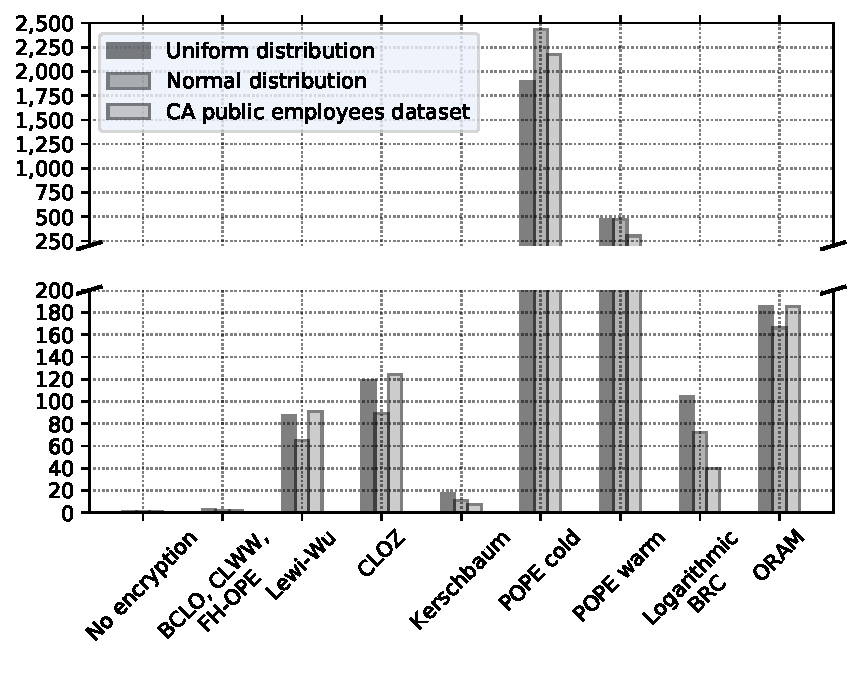
\includegraphics[width=0.6\textwidth]{protocol-charts-qios}
			\caption{
				Query stage number of I/O requests \\
				\hyperlink{frame:ore}{\beamerreturnbutton{Back to ORE}}
			}
		\end{figure}

	\end{frame}

	\begin{frame}[label={frame:appendix:oram}]

		\frametitle{Access pattern and ORAM}

		\justifying%

		\textbf{Access pattern} is a sequence of memory accesses \oramProgram{}, where each access consists of the memory \emph{location} $o$, read \oramRead{} or write \oramWrite{} \emph{operation} and the \emph{data} $d$ to be written.

		Oblivious RAM (ORAM) is a mechanism that hides the accesses pattern.
		More formally, \oram{} is a protocol between the client \client{} (who accesses) and the server \server{} (who stores), with a guarantee that the view of the server is indistinguishable for any two sequences of the same lengths.

		\begin{columns}[T]
			\column{0.475\textwidth}

				\[
					\begin{split}
						\abs{\oramProgram_1}					& = \abs{\oramProgram_2}							\\
						\textsc{View}_\server (\oramProgram_1)	& \cindist \textsc{View}_\server (\oramProgram_2)
					\end{split}
				\]

			\column{0.475\textwidth}

				\procedure[linenumbering]{\oram{} protocol}{
					\textbf{Client \client}											\>														\> \textbf{Server \server}	\\
					%
					\oramProgram{} = \left. (\oramRead, i, \bot) \right|_{i = 1}^5	\> 														\>							\\
					%
					\text{(client state)}											\> \sendmessageboth*[6em]{\algo{ORAM}{\oramProgram}}	\> \text{(server state)}	\\
					%
					\{ d_1, d_2, d_3, d_4, d_5 \}									\>														\>
				}

		\end{columns}

		\vspace*{1ex}

		Square Root ORAM \cite{oram-theory}, Hierarchical ORAM \cite{oram-original}, Binary-Tree ORAM \cite{binary-tree-oram}, Interleave Buffer Shuffle Square Root ORAM \cite{shortest-path-oram}, TP-ORAM \cite{tp-oram}, \textbf{PathORAM} \cite{path-oram} and TaORAM \cite{taostore}.
		\alert{ORAM incurs at least logarithmic overhead in the number of stored records. \cite{oram-original}}

		\begin{flushright}
			\hyperlink{frame:epsolute-motivation}{\beamerreturnbutton{Back to \epsolute{}}}
		\end{flushright}

	\end{frame}

	% chktex-file 1
	% chktex-file 8

	\begin{frame}[fragile,label={frame:appendix:dcpe}]

		\frametitle{Distance Comparison Preserving Encryption algorithms \cite{dcpe}}

		\justifying%

		\newlength{\algSeparationLength}
		\setlength{\algSeparationLength}{5.25em}

		\begin{algorithm}[H]

			\begin{pchstack}

				\procedure[linenumbering]{\algo{KeyGen}{\secparam, \mathbb{S}}}{
					s \sample \mathbb{S}		\\
					\key \sample \bin^\secpar	\\
					\pcreturn (s, \key)
				}

				\hspace*{\algSeparationLength}

				\procedure[linenumbering]{\algo{Enc}{ (s, \key), \vec{m} }}{
					n \sample \bin^\secpar														\\
					\mathsf{coins}_n || \mathsf{coins}_u \gets \algo{prf}{\key, n}	\\
					\vec{n} \sample \algo{Normal}{0, I_d; \mathsf{coins}_n}						\\
					u \sample \algo{Uniform}{0, 1; \mathsf{coins}_u}							\\
					x \gets \frac{s \beta}{4} \cdot \sqrt[d]{u}									\\
					\vec{\delta} \gets \frac{\vec{n}}{\|\vec{n}\|} \cdot x						\\
					\vec{c} \gets s \cdot \vec{m} + \vec{\delta}								\\
					\pcreturn \vec{c}
				}

				\hspace*{\algSeparationLength}

				\procedure[linenumbering]{\algo{Dec}{ (s, \key), (\vec{c}, n) }}{
					\mathsf{coins}_n || \mathsf{coins}_u \gets \algo{prf}{\key, n}	\\
					\vec{n} \sample \algo{Normal}{0, I_d; \mathsf{coins}_n}						\\
					u \sample \algo{Uniform}{0, 1; \mathsf{coins}_u}							\\
					x \gets \frac{s \beta}{4} \cdot \sqrt[d]{u}									\\
					\vec{\delta} \gets \frac{\vec{n}}{\|\vec{n}\|} \cdot x						\\
					\vec{m} \gets \frac{\vec{c} - \vec{\delta}}{s}								\\
					\pcreturn \vec{m}
				}

			\end{pchstack}

			\caption{Distance Comparison Preserving Encryption, adapted from \cite[Algorithm 2]{dcpe}}

		\end{algorithm}

		\begin{flushright}
			\hyperlink{frame:dcpe}{\beamerreturnbutton{Back to Private \knn{}}}
		\end{flushright}

	\end{frame}
